\documentclass{standalone}
\usepackage{tikz}
\usetikzlibrary{patterns, positioning}
\usepackage[sfdefault]{ClearSans} %% option 'sfdefault' activates Clear Sans as the default text font
\usepackage[T1]{fontenc}

\begin{document}
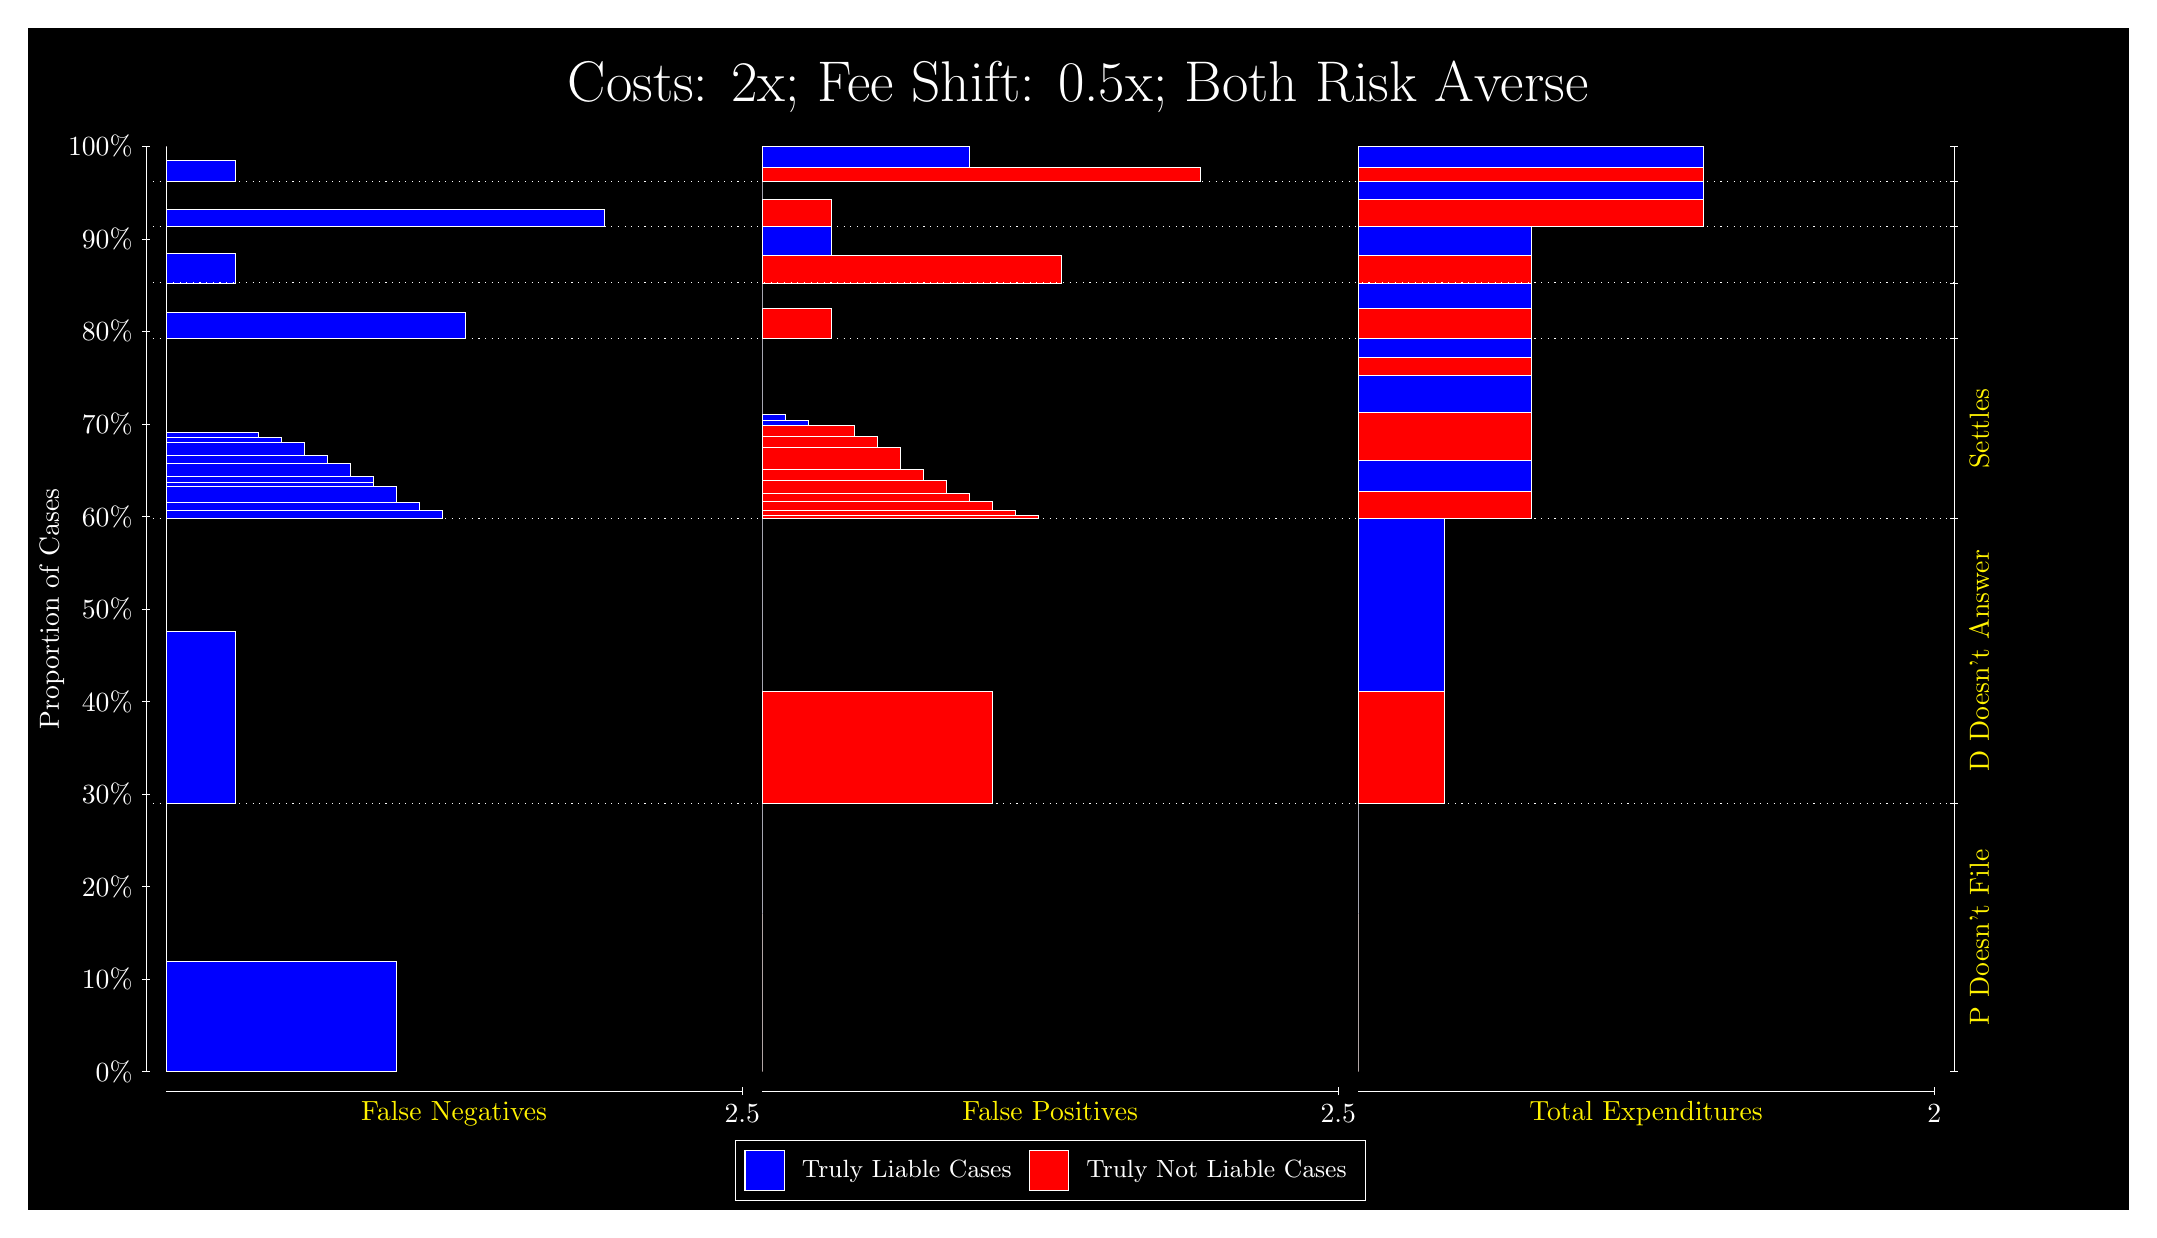
\begin{tikzpicture}
\draw[fill=black] (0,0) rectangle (26.667,15);
\draw[text=white] (0,13.5) rectangle (26.667,15) node[midway] {\huge Costs: 2x; Fee Shift: 0.5x; Both Risk Averse};
\draw[white, very thin] (1.5,1.75) -- (1.5,13.5);
\node[rotate=90, text=white, anchor=center] at (0.3, 7.625) {Proportion of Cases};
\draw[white, very thin] (1.45,1.75) -- (1.55,1.75);
\node[text=white, anchor=east] at (1.45, 1.75) {0\%};
\draw[white, very thin] (1.45,2.925) -- (1.55,2.925);
\node[text=white, anchor=east] at (1.45, 2.925) {10\%};
\draw[white, very thin] (1.45,4.1) -- (1.55,4.1);
\node[text=white, anchor=east] at (1.45, 4.1) {20\%};
\draw[white, very thin] (1.45,5.275) -- (1.55,5.275);
\node[text=white, anchor=east] at (1.45, 5.275) {30\%};
\draw[white, very thin] (1.45,6.45) -- (1.55,6.45);
\node[text=white, anchor=east] at (1.45, 6.45) {40\%};
\draw[white, very thin] (1.45,7.625) -- (1.55,7.625);
\node[text=white, anchor=east] at (1.45, 7.625) {50\%};
\draw[white, very thin] (1.45,8.8) -- (1.55,8.8);
\node[text=white, anchor=east] at (1.45, 8.8) {60\%};
\draw[white, very thin] (1.45,9.975) -- (1.55,9.975);
\node[text=white, anchor=east] at (1.45, 9.975) {70\%};
\draw[white, very thin] (1.45,11.15) -- (1.55,11.15);
\node[text=white, anchor=east] at (1.45, 11.15) {80\%};
\draw[white, very thin] (1.45,12.325) -- (1.55,12.325);
\node[text=white, anchor=east] at (1.45, 12.325) {90\%};
\draw[white, very thin] (1.45,13.5) -- (1.55,13.5);
\node[text=white, anchor=east] at (1.45, 13.5) {100\%};

\draw[white, very thin] (24.457,1.75) -- (24.457,13.5);
\draw[white, very thin] (24.407,1.75) -- (24.507,1.75);
\node[anchor=west] at (24.407, 1.75) {};
\draw[white, very thin] (24.407,5.1575) -- (24.507,5.1575);
\node[anchor=west] at (24.407, 5.1575) {};
\draw[white, very thin] (24.407,8.7727) -- (24.507,8.7727);
\node[anchor=west] at (24.407, 8.7727) {};
\draw[white, very thin] (24.407,11.059) -- (24.507,11.059);
\node[anchor=west] at (24.407, 11.059) {};
\draw[white, very thin] (24.407,11.766) -- (24.507,11.766);
\node[anchor=west] at (24.407, 11.766) {};
\draw[white, very thin] (24.407,12.486) -- (24.507,12.486);
\node[anchor=west] at (24.407, 12.486) {};
\draw[white, very thin] (24.407,13.05) -- (24.507,13.05);
\node[anchor=west] at (24.407, 13.05) {};
\draw[white, very thin] (24.407,13.5) -- (24.507,13.5);
\node[anchor=west] at (24.407, 13.5) {};

\draw[white, very thin, fill=blue] (1.75,1.75) rectangle (4.6775,3.1509);
\draw[white, very thin, fill=red] (1.75,3.1509) rectangle (1.75,5.1575);
\draw[white, very thin, fill=blue] (1.75,5.1575) rectangle (2.6283,7.3454);
\draw[white, very thin, fill=red] (1.75,7.3454) rectangle (1.75,8.7727);
\draw[white, very thin, fill=blue] (1.75,8.7727) rectangle (5.2631,8.879);
\draw[white, very thin, fill=blue] (1.75,8.879) rectangle (4.9703,8.9795);
\draw[white, very thin, fill=blue] (1.75,8.9795) rectangle (4.6775,9.1812);
\draw[white, very thin, fill=blue] (1.75,9.1812) rectangle (4.3848,9.237);
\draw[white, very thin, fill=blue] (1.75,9.237) rectangle (4.3848,9.3105);
\draw[white, very thin, fill=blue] (1.75,9.3105) rectangle (4.092,9.469);
\draw[white, very thin, fill=blue] (1.75,9.469) rectangle (3.7993,9.5719);
\draw[white, very thin, fill=blue] (1.75,9.5719) rectangle (3.5065,9.737);
\draw[white, very thin, fill=blue] (1.75,9.737) rectangle (3.2138,9.8104);
\draw[white, very thin, fill=blue] (1.75,9.8104) rectangle (2.921,9.8729);
\draw[white, very thin, fill=red] (1.75,9.8729) rectangle (1.75,11.059);
\draw[white, very thin, fill=blue] (1.75,11.059) rectangle (5.5558,11.387);
\draw[white, very thin, fill=red] (1.75,11.387) rectangle (1.75,11.766);
\draw[white, very thin, fill=blue] (1.75,11.766) rectangle (2.6283,12.139);
\draw[white, very thin, fill=red] (1.75,12.139) rectangle (1.75,12.486);
\draw[white, very thin, fill=blue] (1.75,12.486) rectangle (7.3123,12.705);
\draw[white, very thin, fill=red] (1.75,12.705) rectangle (1.75,13.05);
\draw[white, very thin, fill=blue] (1.75,13.05) rectangle (2.6283,13.317);
\draw[white, very thin, fill=red] (1.75,13.317) rectangle (1.75,13.5);
\draw[white, very thin, fill=red] (9.3189,1.75) rectangle (9.3189,3.7566);
\draw[white, very thin, fill=blue] (9.3189,3.7566) rectangle (9.3189,5.1575);
\draw[white, very thin, fill=red] (9.3189,5.1575) rectangle (12.246,6.5848);
\draw[white, very thin, fill=blue] (9.3189,6.5848) rectangle (9.3189,8.7727);
\draw[white, very thin, fill=red] (9.3189,8.7727) rectangle (12.832,8.8179);
\draw[white, very thin, fill=red] (9.3189,8.8179) rectangle (12.539,8.8739);
\draw[white, very thin, fill=red] (9.3189,8.8739) rectangle (12.246,8.9983);
\draw[white, very thin, fill=red] (9.3189,8.9983) rectangle (11.954,9.0988);
\draw[white, very thin, fill=red] (9.3189,9.0988) rectangle (11.661,9.261);
\draw[white, very thin, fill=red] (9.3189,9.261) rectangle (11.368,9.4023);
\draw[white, very thin, fill=red] (9.3189,9.4023) rectangle (11.075,9.6795);
\draw[white, very thin, fill=red] (9.3189,9.6795) rectangle (10.783,9.8148);
\draw[white, very thin, fill=red] (9.3189,9.8148) rectangle (10.49,9.9592);
\draw[white, very thin, fill=blue] (9.3189,9.9592) rectangle (9.9044,10.022);
\draw[white, very thin, fill=blue] (9.3189,10.022) rectangle (9.6116,10.095);
\draw[white, very thin, fill=blue] (9.3189,10.095) rectangle (9.3189,11.059);
\draw[white, very thin, fill=red] (9.3189,11.059) rectangle (10.197,11.439);
\draw[white, very thin, fill=blue] (9.3189,11.439) rectangle (9.3189,11.766);
\draw[white, very thin, fill=red] (9.3189,11.766) rectangle (13.125,12.113);
\draw[white, very thin, fill=blue] (9.3189,12.113) rectangle (10.197,12.486);
\draw[white, very thin, fill=red] (9.3189,12.486) rectangle (10.197,12.831);
\draw[white, very thin, fill=blue] (9.3189,12.831) rectangle (9.3189,13.05);
\draw[white, very thin, fill=red] (9.3189,13.05) rectangle (14.881,13.233);
\draw[white, very thin, fill=blue] (9.3189,13.233) rectangle (11.954,13.5);
\draw[white, very thin, fill=red] (16.888,1.75) rectangle (16.888,3.7566);
\draw[white, very thin, fill=blue] (16.888,3.7566) rectangle (16.888,5.1575);
\draw[white, very thin, fill=red] (16.888,5.1575) rectangle (17.986,6.5848);
\draw[white, very thin, fill=blue] (16.888,6.5848) rectangle (17.986,8.7727);
\draw[white, very thin, fill=red] (16.888,8.7727) rectangle (19.083,9.1153);
\draw[white, very thin, fill=blue] (16.888,9.1153) rectangle (19.083,9.5123);
\draw[white, very thin, fill=red] (16.888,9.5123) rectangle (19.083,10.122);
\draw[white, very thin, fill=blue] (16.888,10.122) rectangle (19.083,10.586);
\draw[white, very thin, fill=red] (16.888,10.586) rectangle (19.083,10.821);
\draw[white, very thin, fill=blue] (16.888,10.821) rectangle (19.083,11.059);
\draw[white, very thin, fill=red] (16.888,11.059) rectangle (19.083,11.439);
\draw[white, very thin, fill=blue] (16.888,11.439) rectangle (19.083,11.766);
\draw[white, very thin, fill=red] (16.888,11.766) rectangle (19.083,12.113);
\draw[white, very thin, fill=blue] (16.888,12.113) rectangle (19.083,12.486);
\draw[white, very thin, fill=red] (16.888,12.486) rectangle (21.279,12.831);
\draw[white, very thin, fill=blue] (16.888,12.831) rectangle (21.279,13.05);
\draw[white, very thin, fill=red] (16.888,13.05) rectangle (21.279,13.233);
\draw[white, very thin, fill=blue] (16.888,13.233) rectangle (21.279,13.5);
\draw[white, dotted] (1.5,5.1575) -- (24.457,5.1575);
\draw[white, dotted] (1.5,8.7727) -- (24.457,8.7727);
\draw[white, dotted] (1.5,11.059) -- (24.457,11.059);
\draw[white, dotted] (1.5,11.766) -- (24.457,11.766);
\draw[white, dotted] (1.5,12.486) -- (24.457,12.486);
\draw[white, dotted] (1.5,13.05) -- (24.457,13.05);
\draw[white, very thin] (1.75,1.5) -- (9.0689,1.5);
\node[text=yellow, anchor=north] at (5.4094, 1.5) {False Negatives};
\draw[white, very thin] (9.0689,1.45) -- (9.0689,1.55);
\node[text=white, anchor=north] at (9.0689, 1.45) {2.5};

\draw[white, very thin] (9.3189,1.5) -- (16.638,1.5);
\node[text=yellow, anchor=north] at (12.978, 1.5) {False Positives};
\draw[white, very thin] (16.638,1.45) -- (16.638,1.55);
\node[text=white, anchor=north] at (16.638, 1.45) {2.5};

\draw[white, very thin] (16.888,1.5) -- (24.207,1.5);
\node[text=yellow, anchor=north] at (20.547, 1.5) {Total Expenditures};
\draw[white, very thin] (24.207,1.45) -- (24.207,1.55);
\node[text=white, anchor=north] at (24.207, 1.45) {2};

\node[text=yellow, centered, rotate=90] at (24.777, 3.4538) {P Doesn't File};
\node[text=yellow, centered, rotate=90] at (24.777, 6.9651) {D Doesn't Answer};
\node[text=yellow, centered, rotate=90] at (24.777, 9.916) {Settles};





\draw (12.978300999999998,1.5) node[draw=none] (baseCoordinate) {};
\begin{scope}[align=center]
        \matrix[scale=0.5, draw=white, below=0.5cm of baseCoordinate, nodes={draw}, column sep=0.1cm]{
            \node[rectangle, draw, minimum width=0.5cm, minimum height=0.5cm, fill=blue] {}; &
            \node[draw=none, font=\small, text=white] (B) {Truly Liable Cases}; &
            \node[rectangle, draw, minimum width=0.5cm, minimum height=0.5cm, fill=red] {}; &
            \node[draw=none, font=\small, text=white] (B) {Truly Not Liable Cases}; \\
            };
\end{scope}

\end{tikzpicture}
\end{document}